\subsection{AL in cold atoms}
AL was originally introduced in a condensed-matter system, for example, electrons in a disordered crystal and spins in a disordered field. But there are a number of difficulties for observing AL in a condensed-matter system. The interaction between electrons is hard to change, there are no good methods to directly measure the wave function of electrons in a solid. In contrast, cold atoms is an ideal platform to study AL. The interaction between neutral atoms can be tuned negligible, the wave function of atoms can be directly measured by absorption imaging and the optical dipole potential has been used to generate optical lattices.

1D AL was first observed in cold atoms in 2008 \cite{billy2008direct,roati2008anderson}. In both the experiments, the disordered potential was realized using optical dipole potentials. In \cite{billy2008direct}, optical speckle potential from far-blue-detuned light was used. The statistical properties of the optical speckle was well studied in the 1970s \cite{goodman2007speckle}. In \cite{roati2008anderson}, one-dimensional optical lattice perturbed by a second, weak incommensurate lattice yields localization effect. And the dependence of localization on strength of the disorder was studied. Later in 2011, 3D AL was realized \cite{kondov2011three}. The researchers observed three-dimensional AL of noninteracting ultracold atoms by allowing a spin-polarized atomic Fermi gas to expand into a disordered
potential. In this experiment, the mobility edge was extracted. In lower dimensions, actual mobility edge does not exist but quasi-mobility edge as a function of the correlation length of the disordered potential has significant effects on the spread of the wave function \cite{sanchez2007anderson,billy2008direct}.

\begin{figure}[htbp]
    \centering
    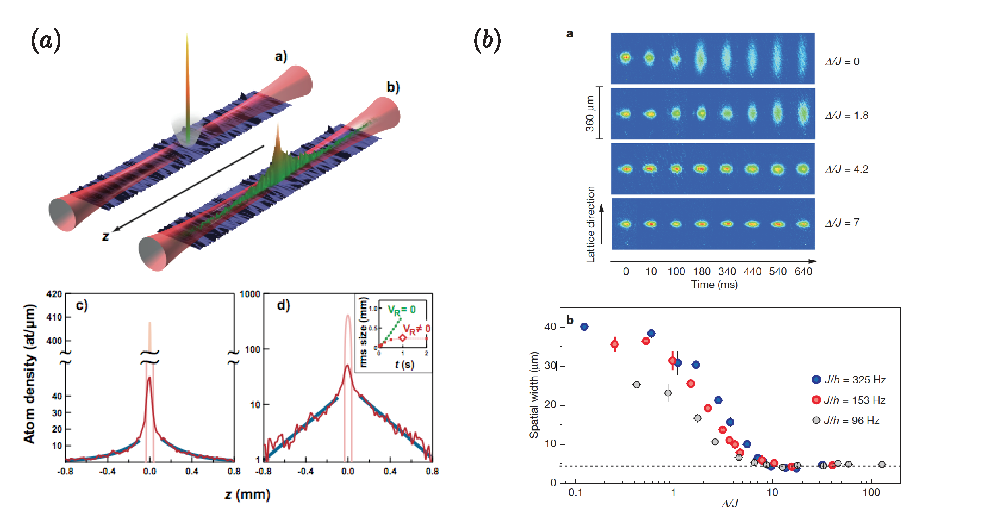
\includegraphics[width=\textwidth]{Chapter3_secs/AL2.pdf}
    \caption{First 1D AL experiments in cold atoms. (a). Fig.~(1) in \cite{billy2008direct}, Observation of the exponential localization. (b). Fig.~(2) in \cite{roati2008anderson}, Probing the localization with transport. }
    \label{fig:AL2}
\end{figure}

As shown in Fig.~(\ref{fig:AL2})(a), a BEC is made in a hybrid trap consisting of a dipole trap and a magnetic trap providing longitudinal confinement. 1d optical speckle potential along the dipole trap was added. At t=0, the magnetic trap was turned off and the BEC started expanding due to the repulsive interaction of atoms. Without the optical speckle, the width of the atoms grow linearly in time, and as they expand, the density drops and the interaction becomes negligible. In this process, the interaction is converted into kinetic energy and the mean-field energy determines $k_{max}$ in the momentum distribution after expansion. It is predicted in theory \cite{sanchez2007anderson},  for a speckle potential with intensity correlation length $\sigma_R$, when $k_{max}\sigma_R<1$, the localized wave function has a tail that exponentially decays. This is a feature of AL. When $k_{max}\sigma_R>1$, the density profiles should have algebraic wings. $\sigma_R$ determines the quasi-mobility edge in 1D.

In Fig.~(\ref{fig:AL2})(b), 1D AL was observed in a one-dimensional quasi-periodic lattice. The system is described by an Anbry-Andr\'{e} model \cite{aubry1980analyticity,harper1955single}
\begin{equation}
    \hat{H} = J\sum_m (\dyad{w_m}{w_{m+1}} + \dyad{w_m}{w_{m+1}}) + \Delta\sum_m \cos{2\pi\beta m + \phi}\dyad{w_m}{w_m}.
\end{equation}
$\ket{w_m}$ is the Wannier function at lattice site m, $J$ is the tunnelling energy and $\Delta$ is the strength of the disorder potential. The researcher make the noninteracting BEC expand along the 1D lattice, and measure the spatial density of the atoms as a function of time and the disorder strength. As the ratio of the disorder strength and the tunnelling strength, $\Delta/J$ goes above a critical value, they observed a crossover between ballistic expansion of the BEC and no expansion. They demonstrated that the system has the feature as that in the case of purely-random disorder in higher dimensions. 

These research works paved the way for more sophisticated AL studies in cold atoms and enables the interplay between AL and other well studied topics in cold atoms, for example, spin-orbit coupling.